Markov Chain Monte Carlo (MCMC) methods \cite{Geyer_2011} are a class of algorithms that are used to sample a probability distribution that is analytically intractable, or just very complex. A Markov Chain is constructed, that has the same distribution as the target distribution, and recording the chain, the target distribution is uncovered. Since MCMC methods only uncover the true target distribution for very large chain lengths, or even infinite length, a practical convergence criterion is needed to numerically approximate the target multidimensional distributions. We know, that target distributions are calculated via solving integrals of the form \ref{eq:Bayes_with_intractable_term}, so MCMC methods are a likely choice to base further evaluations on. An example of this is depicted in the following figure, where an algorithm is shown that lets the test distribution converge towards the target distribution using the metropolis hastings algorithm.
\begin{figure}[h!]%Metropolis Hastings Convergence Example
	\centering
	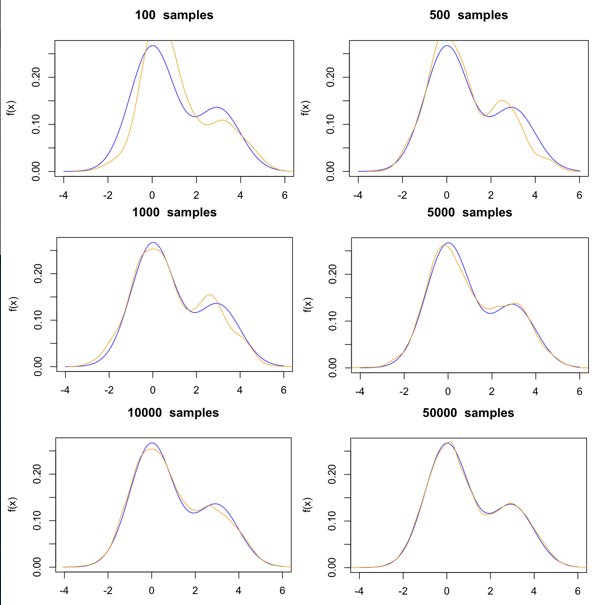
\includegraphics[width=4in]{img/05_6/MetropolisHastingsConvergence.png}
	\caption[Metropolis Hastings Convergence Example]
	{Convergence of the Metropolis Hastings algorithm as an example for Markov chain Monte Carlo methods approximating the target distribution of a bayesian problem. It is clear that more samples lead to a better approximation of the target distribution.}
\end{figure}
A necessary precondition is that the probability density of the target random variable is given up to a constant. If the integral is intractable, MCMC methods can evaluate the integral statistically by generating an ensemble of chains starting at arbitrarily chosen points. A chain is a stochastic process, that moves around randomly on this high dimensional probability surface where moves are generated via Monte Carlo sampling, and then an evaluation of the contribution of this place to the integral is carried out. If the posterior mass is low in some regions, the chain will move away faster from this location, while on the other hand it will spend more moves in regions with higher posterior mass. These Markov chains then have an equilibrium distribution proportional to the target distribution. MCMC methods, even though outperforming generic Monte Carlo algorithms, still suffer from the curse of dimensionality, where regions of higher probability tend to stretch due to a high number of dimensions. Regions with higher probability mass then do not get the proportion of moves necessary in the faster scaling volume of high dimensional space, and contribute less to the solution. This method also implies a problem of when to accept a chain to be converged to a stationary distribution with a reasonable error. Here, the term of rapid mixing becomes important, describing the phenomenon of stationary distributions being reached quickly while starting from arbitrary positions, highlighting the need to sample several chains for non-variational inference algorithms. An extension of the central limit theorem, the Markov chain central limit theorem \cite{Andrieu_2003}, states that for a sequence of random elements forming a Markov chain with the Markov property, the mean of the Markov chain will tend towards a normal distribution. Formally, we have a sequence of random elements $X_1, X_2, X_3, ...$ of some set $\mathcal{X}$ forming the Markov chain with a stationary probability distribution. Also, the initial distribution of the process, the distribution leading to $X_1$ has to be stationary, which entails that $X_1, X_2, X_3, ...$ are identically distributed. Then, the Markov property is necessary, and we need a measurable real-valued function $g$ with $var(g(X_1))<+\infty$.
\begin{subequations}%markov chain central limit theorem prerequisites
	\label{eq:markov chain central limit theorem prerequisites}
	\begin{align}
	\mu = \mathbb{E}(g(X_1)),                                                    \label{eq:mean of initial markov chain step} \\
	\sigma^2 = var(g(X_1)) + 2\sum_{k=1}^{\infty}cov(g(X_1), g(X_{1+k})),         \label{eq:variance markov steps} \\
	\hat{\mu}_n = \frac{1}{n} \sum_{k=1}^{n}g(X_k).                               \label{eq:expected mean markov process}
	\end{align}
\end{subequations}
For $n \to \infty$, we find:
\begin{equation}%markov chain convergence
	\label{eq:markov chain convergence}
	\sqrt{n}(\hat{\mu_n}-\mu) \to \mathcal{N}(0, \sigma^2),         
\end{equation}
resulting in an important feature for convergence. Furthermore, a solution to the curse of dimensionality would be to accept higher autocorrelation and expensive computations by using smaller steps of the chain, which is impractical. More sophisticated methods, like Hamiltonian Monte Carlo reduce autocorrelation while keeping the chain in the desired regions of the probability surface. 

\subsubsection{Hamiltonian Monte Carlo}
Hamiltonian Monte Carlo (HMC) \cite{Duane_1987} is a MCMC method that applies derivatives of the density function to generate efficient transitions when approximating the posterior. The dynamics of the chain is given by Hamiltons equations of motion. The Hamiltonian dynamics simulation is carried out using numerical integration. To achieve this, HMC uses auxiliary momentum variables to form a joint density to draw from. 
\begin{equation}%HMC joint density for regular and auxiliar variables
	p(\rho, \theta) = p(\rho | \theta) p(\theta),
\label{eq: HMC joint density for regular and auxiliar variables}
\end{equation}
where $\rho$ are the auxiliary momentan variables, and $\theta$ are the parameters of the model. By choosing the following distribution for $\rho$, it becomes independent of $\theta$.
\begin{equation}%HMC independent auxiliary variables
	\rho \thicksim \mathcal{N}(0,M).
\label{eq:HMC_independent_auxiliary_variables}
\end{equation}
Here, $M$ is the Euclidian metric, which is just a transformation of parameter space to enhance the efficiency of sampling. The joint density of auxiliary and regular parameters then leads to the combined Hamiltonian
\begin{equation}%HMC Hamiltonian
	H(\rho,\theta) = -log(p(\rho, \theta)) = -log(p(\rho | \theta)) - log(p(\theta)) = T(\rho | \theta) + V(\theta),
\label{eq: HMC Hamiltonian}
\end{equation}
where we define $T(\rho | \theta)$ and $V(\theta)$ as kinetic energy and potential energy respectively, directly analogous to physics. in statistics we find that $T(\rho | \theta) = -log(p(\rho | \theta))$ and $V(\theta) = log(p(\theta))$. The potential energy is often in a statistical context regarded as a log density. From this on, we can use Hamilton´s equations to find find the momentum needed for state transitions. The momentum parameter values are independently drawn using \ref{eq:HMC_independent_auxiliary_variables}, so that momentum is changing across iterations. We use
\begin{subequations}%HMC Hamiltonian equations
	\label{eq:HMC Hamiltonian equations}
	\begin{align}
	\frac{d\theta}{dt} = \frac{\partial H}{\partial \rho} = \frac{\partial T}{\partial \rho},         \label{eq:HMC parameter Hamilton equation} \\
	\frac{d\rho}{dt} = -\frac{\partial H}{\partial \theta} = \frac{\partial T}{\partial \theta} - \frac{\partial V}{\partial \theta} = - \frac{\partial V}{\partial \theta},         \label{eq:HMC auxiliary Hamiltonian equation}
	\end{align}
\end{subequations}
where we have recognized the momentum density $\partial T/\partial \theta$ to be zero, due to the independence of momentum density and target density. This two-state differential equation can then be solved using many integrators. We will discuss the Leapfrog integrator here, since it is most widely used in HMC implementations. In general the Leapfrog integrator uses half integer time steps to calculate velocities and integer time steps to calculate  positions, which pans out to the following updating equations:
\begin{subequations}%HMC Leapfrog update equations
	\label{eq:HMC Leapfrog update equations}
	\begin{align}
	\rho \leftarrow \rho - \frac{\epsilon}{2}\frac{\partial V}{\partial \theta},         \label{eq:LF update rule momentum} \\
	\theta \leftarrow \theta + \epsilon M^{-1}\rho.         \label{eq:LF update rule pamaeters}  
	\end{align}
\end{subequations}
Here, the first update rule is carried out twice, once at the start of a timestep and once at the end. The symplectic Leapfrog integrator has a $\mathcal{O}(\epsilon^3)$ error per step, and globally an error of $\mathcal{O}(\epsilon^2)$. Following a calculated transition, the Metropolis acceptance step begins, where evaluation of the energy of the Hamiltonian leads to accepting the proposed step, or throwing this set of parameters away. The probability of keeping a step can be calculated via
\begin{equation}%Metropolis Acceptance probability of a HMC step
	min(1, exp(H(\rho, \theta))-exp(H(\rho^*, \theta^*))),
\label{eq: Metropolis Acceptance probability of a HMC step.}
\end{equation}
where $\rho^*, \theta^*$ are the proposed values and $\rho, \theta$ the origin of the proposed transition. We do not have to implement HMC by ourself. We can use probabilistic programming languages such as stan. For that, we onl yghave to define the unnormalized posterior density and the approximation thereof is carried out by stan.

\subsubsection{Stochastic Gradient Ascent}
\label{sec:stochastic_gradient_ascent}
Stans variational inference algorithm, Automatic Differentiation Variational Inference \cite{Kucukelbir_2015}, optimizes the ELBO in real-coordinate space. The stochastic gradient ascent obtains unbiased, yet noisy gradients through automatic differentiation and evaluates the ELBO using Monte Carlo integration. Along these gradients, the algorithm ascends using a sequence of adaptive stepsizes. Typically, in practice, the ELBO is sampled with around 100 samples, so that the true ELBO value can be approximated with reasonably high confidence. The ELBO is only evaluated every few iterations, to save computation time, but inside high dimensional manifolds, this seems not to be a problem in practice \cite{stan_manual}. The gradients are also approximated using Monte Carlo Integration, but usually only one sample is drawn, as experience has shown that, while remaining high computational efficiency, stochastic gradient ascent is capable of following such gradients nonetheless. Adaptive step sizes are optimized during a warmup phase where a good value for the single exposed parameter is selected from values spanning multiple orders of magnitude \cite{stan_manual}. This parameter is then used in combination with a finite memory version of adaGrad \cite{Duchi_2011}. In the end, every calculation needs to asses convergence, but since there are no closed form analytical expressions available, the progression of the ELBO values has to be tracked. Using a rolling window, which is heuristically determined, in which the average and median change of the ELBO are computed, we assume convergence if either of those values has fallen below a certain threshold. 